\documentclass[10pt]{article}
\usepackage{tikz}
\usepackage{amsmath}
\usepackage{fourier}
\usepackage{listings}
\usepackage{enumitem}
\renewcommand\theenumi{\textbf{Q\arabic{enumi}}}
\renewcommand{\vec}[1]{\ensuremath{\boldsymbol{#1}}}

\newcommand\tikzbox{\begin{tikzpicture}[baseline=(current bounding box.east)] \draw (0,0) rectangle (2.2in, 0.3in);\end{tikzpicture}}

\DeclareMathOperator{\Si}{Si}
\DeclareMathOperator{\Cin}{Cin}
\DeclareMathOperator{\Ci}{Ci}

\newcommand{\mks}[1]{\hfill
[\textbf{\small {#1}}]
}

\oddsidemargin -0.25in \evensidemargin -0.5in \topmargin
-1in \textheight 9.5in \textwidth 7in

\begin{document}


\begin{tikzpicture}[remember picture,overlay]
\node [xshift=0.75in,yshift=-0.4in]  at (current page.north west)
[text width=7cm,thick,draw=black!80,below right]
{
Name:\\
Student number:
};
\end{tikzpicture}

\begin{tikzpicture}[remember picture,overlay]
\node [xshift=1in,yshift=-0.4in]  at (current page.north)
[text width=7cm,thick,draw=black!80,below]
{
Grader's name:\\
Grader's student number:

};
\end{tikzpicture}

\begin{tikzpicture}[remember picture,overlay]
\node [xshift=-.75in,yshift=-0.4in]  at (current page.north east)
[text width=2.1cm,thick,draw=black!80,below left]
{
Marks:$\qquad/15$\\
Revised:

};
\end{tikzpicture}




\begin{center}
\noindent{Department of Electronic and Telecommunication Engineering, University of Moratuwa, Sri Lanka}\\
{\large EN1060 Signals and Systems---Quiz 01}\\
{\today}
\vspace{.1in}
\end{center}

\noindent \textbf{Instructions:} Answer \textbf{all} the questions in the given space. This is an open-book quiz. Time: 15 minutes. \\
\begin{tikzpicture}
\draw (0in,0in) -- (\textwidth,0in);
\end{tikzpicture}

\begin{enumerate}[leftmargin=*]

\item Plot
    $
        x(t) = A\cos(\omega_0t+ \phi)
    $
    where \mks{2}

  \noindent  \begin{tabular}{cc}
        $A=1$, $\omega_0 = 1\:\mathrm{rad/s}$, $\phi = 0$ & $A=1$, $\omega_0 = 1\:\mathrm{rad/s}$, $\phi = -\pi/2$ \\
        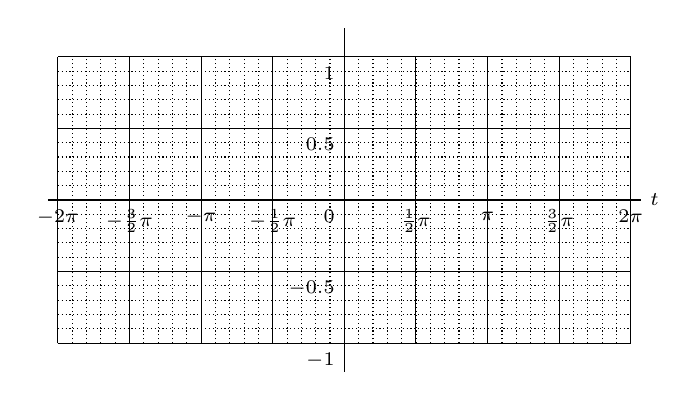
\begin{tikzpicture}[xscale=0.579, yscale=1.818]
	\def\piv{3.1416}
	\coordinate (o) at (0,0);
	\draw (o) ++(-6.5,0) -- ++(13, 0) node [anchor=west] {\scriptsize $t$};
	\draw (o) ++(0,-1.2) -- ++(0, 2.4);% node [anchor=south] {\scriptsize $x(t)$};	
	
	\foreach \y in {-1, -0.9, ..., 1}
	{
		\draw[thin, densely dotted] (-2*\piv, \y) -- ++(4*\piv, 0);
	}	

	\foreach \x in {- 6.2832, -5.9690, ...,  6.2832}
	{
		\draw[thin, densely dotted]  (\x, -1) -- ++(0,2);
	}		
	
	
	\foreach \x/\v in {-2*\piv/-2, -1.5*\piv/-\frac{3}{2}, -1*\piv/-, -0.5*pi/{-\frac{1}{2}},  0.5*\piv/\frac{1}{2}, 1*\piv/, 1.5*\piv/\frac{3}{2}, 2*\piv/2}
	{
		\draw (\x, -1) -- ++(0,2);
		\node at (\x, 0) [anchor=north, minimum height=0.4cm] {\scriptsize $ \v\pi$};
	}
	\foreach \y in {-1, -0.5, 0, 0.5, 1}
	{
		\draw (-2*\piv, \y) -- ++(4*\piv, 0);
		\node  at (0, \y) [anchor=north east] {\scriptsize $ \y $};
	}

\end{tikzpicture}  & 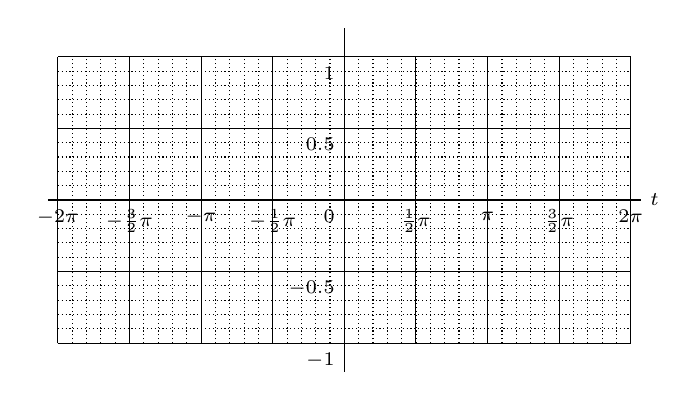
\begin{tikzpicture}[xscale=0.579, yscale=1.818]
	\def\piv{3.1416}
	\coordinate (o) at (0,0);
	\draw (o) ++(-6.5,0) -- ++(13, 0) node [anchor=west] {\scriptsize $t$};
	\draw (o) ++(0,-1.2) -- ++(0, 2.4);% node [anchor=south] {\scriptsize $x(t)$};	
	
	\foreach \y in {-1, -0.9, ..., 1}
	{
		\draw[thin, densely dotted] (-2*\piv, \y) -- ++(4*\piv, 0);
	}	

	\foreach \x in {- 6.2832, -5.9690, ...,  6.2832}
	{
		\draw[thin, densely dotted]  (\x, -1) -- ++(0,2);
	}		
	
	
	\foreach \x/\v in {-2*\piv/-2, -1.5*\piv/-\frac{3}{2}, -1*\piv/-, -0.5*pi/{-\frac{1}{2}},  0.5*\piv/\frac{1}{2}, 1*\piv/, 1.5*\piv/\frac{3}{2}, 2*\piv/2}
	{
		\draw (\x, -1) -- ++(0,2);
		\node at (\x, 0) [anchor=north, minimum height=0.4cm] {\scriptsize $ \v\pi$};
	}
	\foreach \y in {-1, -0.5, 0, 0.5, 1}
	{
		\draw (-2*\piv, \y) -- ++(4*\piv, 0);
		\node  at (0, \y) [anchor=north east] {\scriptsize $ \y $};
	}

\end{tikzpicture}  \\
    \end{tabular}


\item Plot
    $
        x(t) = A\sin(\omega_0t+ \phi)
    $
    where \mks{2}

  \noindent  \begin{tabular}{cc}
        $A=1$, $\omega_0 = 2\:\mathrm{rad/s}$, $\phi = 0$ & $A=1$, $\omega_0 = 2\:\mathrm{rad/s}$, $\phi = -\pi/2$ \\
        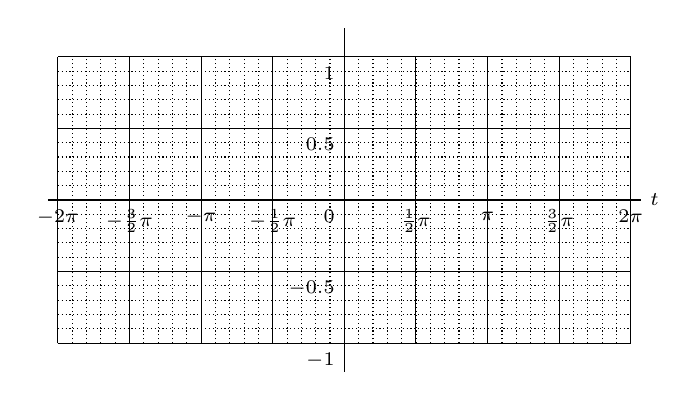
\begin{tikzpicture}[xscale=0.579, yscale=1.818]
	\def\piv{3.1416}
	\coordinate (o) at (0,0);
	\draw (o) ++(-6.5,0) -- ++(13, 0) node [anchor=west] {\scriptsize $t$};
	\draw (o) ++(0,-1.2) -- ++(0, 2.4);% node [anchor=south] {\scriptsize $x(t)$};	
	
	\foreach \y in {-1, -0.9, ..., 1}
	{
		\draw[thin, densely dotted] (-2*\piv, \y) -- ++(4*\piv, 0);
	}	

	\foreach \x in {- 6.2832, -5.9690, ...,  6.2832}
	{
		\draw[thin, densely dotted]  (\x, -1) -- ++(0,2);
	}		
	
	
	\foreach \x/\v in {-2*\piv/-2, -1.5*\piv/-\frac{3}{2}, -1*\piv/-, -0.5*pi/{-\frac{1}{2}},  0.5*\piv/\frac{1}{2}, 1*\piv/, 1.5*\piv/\frac{3}{2}, 2*\piv/2}
	{
		\draw (\x, -1) -- ++(0,2);
		\node at (\x, 0) [anchor=north, minimum height=0.4cm] {\scriptsize $ \v\pi$};
	}
	\foreach \y in {-1, -0.5, 0, 0.5, 1}
	{
		\draw (-2*\piv, \y) -- ++(4*\piv, 0);
		\node  at (0, \y) [anchor=north east] {\scriptsize $ \y $};
	}

\end{tikzpicture}  & 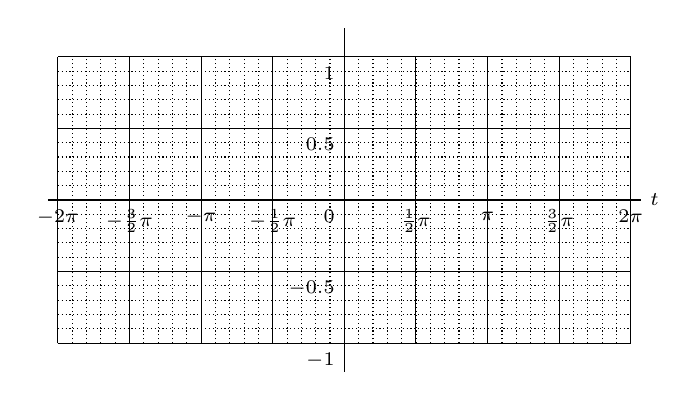
\begin{tikzpicture}[xscale=0.579, yscale=1.818]
	\def\piv{3.1416}
	\coordinate (o) at (0,0);
	\draw (o) ++(-6.5,0) -- ++(13, 0) node [anchor=west] {\scriptsize $t$};
	\draw (o) ++(0,-1.2) -- ++(0, 2.4);% node [anchor=south] {\scriptsize $x(t)$};	
	
	\foreach \y in {-1, -0.9, ..., 1}
	{
		\draw[thin, densely dotted] (-2*\piv, \y) -- ++(4*\piv, 0);
	}	

	\foreach \x in {- 6.2832, -5.9690, ...,  6.2832}
	{
		\draw[thin, densely dotted]  (\x, -1) -- ++(0,2);
	}		
	
	
	\foreach \x/\v in {-2*\piv/-2, -1.5*\piv/-\frac{3}{2}, -1*\piv/-, -0.5*pi/{-\frac{1}{2}},  0.5*\piv/\frac{1}{2}, 1*\piv/, 1.5*\piv/\frac{3}{2}, 2*\piv/2}
	{
		\draw (\x, -1) -- ++(0,2);
		\node at (\x, 0) [anchor=north, minimum height=0.4cm] {\scriptsize $ \v\pi$};
	}
	\foreach \y in {-1, -0.5, 0, 0.5, 1}
	{
		\draw (-2*\piv, \y) -- ++(4*\piv, 0);
		\node  at (0, \y) [anchor=north east] {\scriptsize $ \y $};
	}

\end{tikzpicture}  \\
    \end{tabular}


    \item Plot
    $x[n] = u[n]$, and $x[n] = \delta[n]$.     \mks{1}

  \noindent  \begin{tabular}{cc}
        $u[n]$ & $\delta[n]$\\
        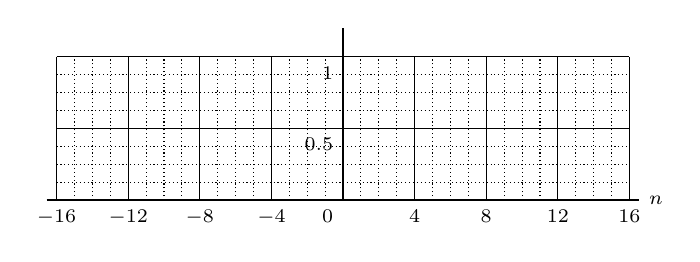
\begin{tikzpicture}[xscale=0.579, yscale=1.818]
	\def\piv{3.1416}
	\coordinate (o) at (0,0);
	\draw (o) ++(-6.5,0) -- ++(13, 0) node [anchor=west] {\scriptsize $n$};
	\draw (o) ++(0,0) -- ++(0, 1.2);% node [anchor=south] {\scriptsize $x[n]$};	
	
	\foreach \y in {0, 0.125, ..., 1}
	{
		\draw[thin, densely dotted] (-2*\piv, \y) -- ++(4*\piv, 0);
	}	

	\foreach \x in {- 6.2832, -5.8905, ...,  6.2832}
	{
		\draw[thin, densely dotted]  (\x, 0) -- ++(0,1);
	}		
	
	
	\foreach \x/\v in {-2*\piv/-16, -1.5*\piv/-12, -1*\piv/-8, -0.5*pi/-4,  0.5*\piv/4, 1*\piv/8, 1.5*\piv/12, 2*\piv/16}
	{
		\draw (\x, 0) -- ++(0,1);
		\node at (\x, 0) [anchor=north, minimum height=0.4cm] {\scriptsize $ \v$};
	}
	\foreach \y in { 0, 0.5, 1}
	{
		\draw (-2*\piv, \y) -- ++(4*\piv, 0);
		\node  at (0, \y) [anchor=north east] {\scriptsize $ \y $};
	}

\end{tikzpicture}  & 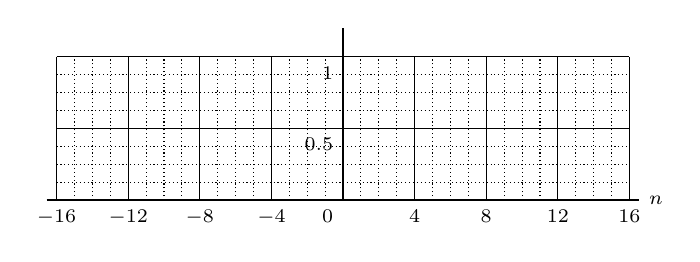
\begin{tikzpicture}[xscale=0.579, yscale=1.818]
	\def\piv{3.1416}
	\coordinate (o) at (0,0);
	\draw (o) ++(-6.5,0) -- ++(13, 0) node [anchor=west] {\scriptsize $n$};
	\draw (o) ++(0,0) -- ++(0, 1.2);% node [anchor=south] {\scriptsize $x[n]$};	
	
	\foreach \y in {0, 0.125, ..., 1}
	{
		\draw[thin, densely dotted] (-2*\piv, \y) -- ++(4*\piv, 0);
	}	

	\foreach \x in {- 6.2832, -5.8905, ...,  6.2832}
	{
		\draw[thin, densely dotted]  (\x, 0) -- ++(0,1);
	}		
	
	
	\foreach \x/\v in {-2*\piv/-16, -1.5*\piv/-12, -1*\piv/-8, -0.5*pi/-4,  0.5*\piv/4, 1*\piv/8, 1.5*\piv/12, 2*\piv/16}
	{
		\draw (\x, 0) -- ++(0,1);
		\node at (\x, 0) [anchor=north, minimum height=0.4cm] {\scriptsize $ \v$};
	}
	\foreach \y in { 0, 0.5, 1}
	{
		\draw (-2*\piv, \y) -- ++(4*\piv, 0);
		\node  at (0, \y) [anchor=north east] {\scriptsize $ \y $};
	}

\end{tikzpicture}  \\
    \end{tabular}


    \item Plot
    $x(t) = u(t)$, and $x(t) = \delta(t)$.     \mks{1}

  \noindent  \begin{tabular}{cc}
        $u(t)$ & $\delta(t)$\\
        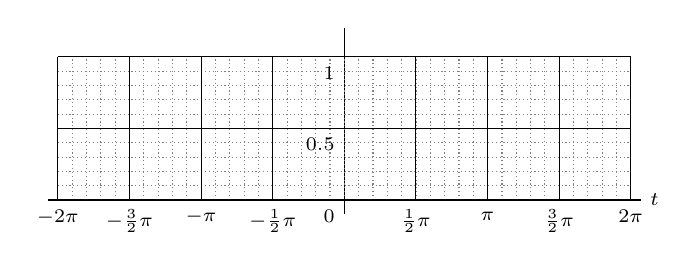
\begin{tikzpicture}[xscale=0.579, yscale=1.818]
	\def\piv{3.1416}
	\coordinate (o) at (0,0);
	\draw (o) ++(-6.5,0) -- ++(13, 0) node [anchor=west] {\scriptsize $t$};
	\draw (o) ++(0,-0.1) -- ++(0, 1.3);% node [anchor=south] {\scriptsize $x(t)$};	
	
	\foreach \y in {0, 0.1, ..., 1}
	{
		\draw[thin, gray, densely dotted] (-2*\piv, \y) -- ++(4*\piv, 0);
	}	

	\foreach \x in {- 6.2832, -5.9690, ...,  6.2832}
	{
		\draw[thin, gray, densely dotted]  (\x, 0) -- ++(0,1);
	}		
	
	
	\foreach \x/\v in {-2*\piv/-2, -1.5*\piv/-\frac{3}{2}, -1*\piv/-, -0.5*pi/{-\frac{1}{2}},  0.5*\piv/\frac{1}{2}, 1*\piv/, 1.5*\piv/\frac{3}{2}, 2*\piv/2}
	{
		\draw (\x, 0) -- ++(0,1);
		\node at (\x, 0) [anchor=north, minimum height=0.4cm] {\scriptsize $ \v\pi$};
	}
	\foreach \y in {0, 0.5, 1}
	{
		\draw (-2*\piv, \y) -- ++(4*\piv, 0);
		\node  at (0, \y) [anchor=north east] {\scriptsize $ \y $};
	}

\end{tikzpicture}  & 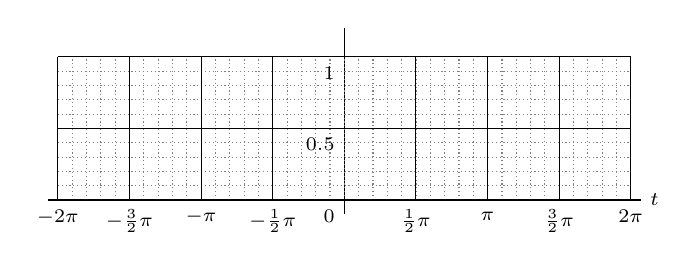
\begin{tikzpicture}[xscale=0.579, yscale=1.818]
	\def\piv{3.1416}
	\coordinate (o) at (0,0);
	\draw (o) ++(-6.5,0) -- ++(13, 0) node [anchor=west] {\scriptsize $t$};
	\draw (o) ++(0,-0.1) -- ++(0, 1.3);% node [anchor=south] {\scriptsize $x(t)$};	
	
	\foreach \y in {0, 0.1, ..., 1}
	{
		\draw[thin, gray, densely dotted] (-2*\piv, \y) -- ++(4*\piv, 0);
	}	

	\foreach \x in {- 6.2832, -5.9690, ...,  6.2832}
	{
		\draw[thin, gray, densely dotted]  (\x, 0) -- ++(0,1);
	}		
	
	
	\foreach \x/\v in {-2*\piv/-2, -1.5*\piv/-\frac{3}{2}, -1*\piv/-, -0.5*pi/{-\frac{1}{2}},  0.5*\piv/\frac{1}{2}, 1*\piv/, 1.5*\piv/\frac{3}{2}, 2*\piv/2}
	{
		\draw (\x, 0) -- ++(0,1);
		\node at (\x, 0) [anchor=north, minimum height=0.4cm] {\scriptsize $ \v\pi$};
	}
	\foreach \y in {0, 0.5, 1}
	{
		\draw (-2*\piv, \y) -- ++(4*\piv, 0);
		\node  at (0, \y) [anchor=north east] {\scriptsize $ \y $};
	}

\end{tikzpicture}  \\
    \end{tabular}


    \item Plot
    $
        x[n] = A\cos(\omega_0n+ \phi)
    $
    where \mks{2}

  \noindent  \begin{tabular}{cc}
        $A=1$, $\omega_0 = \pi/8\:\mathrm{rad/s}$, $\phi = 0$ & $A=1$, $\omega_0 = \pi/8\:\mathrm{rad/s}$, $\phi = -\pi/2$ \\
        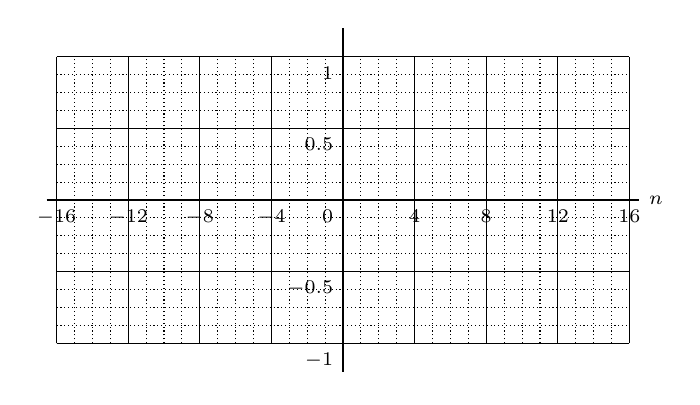
\begin{tikzpicture}[xscale=0.579, yscale=1.818]
	\def\piv{3.1416}
	\coordinate (o) at (0,0);
	\draw (o) ++(-6.5,0) -- ++(13, 0) node [anchor=west] {\scriptsize $n$};
	\draw (o) ++(0,-1.2) -- ++(0, 2.4);% node [anchor=south] {\scriptsize $x[n]$};	
	
	\foreach \y in {-1, -0.875, ..., 1}
	{
		\draw[thin, densely dotted] (-2*\piv, \y) -- ++(4*\piv, 0);
	}	

	\foreach \x in {- 6.2832, -5.8905, ...,  6.2832}
	{
		\draw[thin, densely dotted]  (\x, -1) -- ++(0,2);
	}		
	
	
	\foreach \x/\v in {-2*\piv/-16, -1.5*\piv/-12, -1*\piv/-8, -0.5*pi/-4,  0.5*\piv/4, 1*\piv/8, 1.5*\piv/12, 2*\piv/16}
	{
		\draw (\x, -1) -- ++(0,2);
		\node at (\x, 0) [anchor=north, minimum height=0.4cm] {\scriptsize $ \v$};
	}
	\foreach \y in {-1, -0.5, 0, 0.5, 1}
	{
		\draw (-2*\piv, \y) -- ++(4*\piv, 0);
		\node  at (0, \y) [anchor=north east] {\scriptsize $ \y $};
	}

\end{tikzpicture}  & 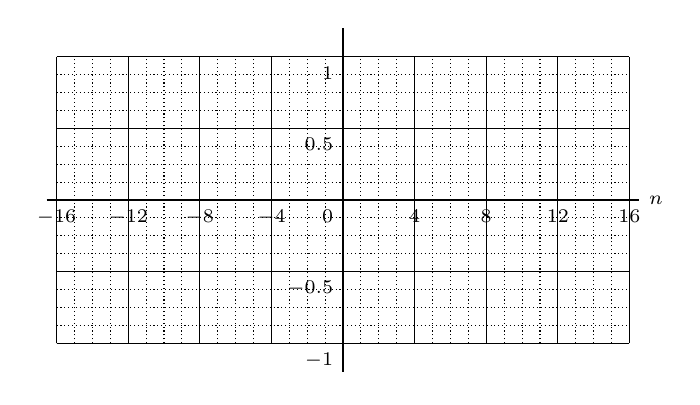
\begin{tikzpicture}[xscale=0.579, yscale=1.818]
	\def\piv{3.1416}
	\coordinate (o) at (0,0);
	\draw (o) ++(-6.5,0) -- ++(13, 0) node [anchor=west] {\scriptsize $n$};
	\draw (o) ++(0,-1.2) -- ++(0, 2.4);% node [anchor=south] {\scriptsize $x[n]$};	
	
	\foreach \y in {-1, -0.875, ..., 1}
	{
		\draw[thin, densely dotted] (-2*\piv, \y) -- ++(4*\piv, 0);
	}	

	\foreach \x in {- 6.2832, -5.8905, ...,  6.2832}
	{
		\draw[thin, densely dotted]  (\x, -1) -- ++(0,2);
	}		
	
	
	\foreach \x/\v in {-2*\piv/-16, -1.5*\piv/-12, -1*\piv/-8, -0.5*pi/-4,  0.5*\piv/4, 1*\piv/8, 1.5*\piv/12, 2*\piv/16}
	{
		\draw (\x, -1) -- ++(0,2);
		\node at (\x, 0) [anchor=north, minimum height=0.4cm] {\scriptsize $ \v$};
	}
	\foreach \y in {-1, -0.5, 0, 0.5, 1}
	{
		\draw (-2*\piv, \y) -- ++(4*\piv, 0);
		\node  at (0, \y) [anchor=north east] {\scriptsize $ \y $};
	}

\end{tikzpicture}  \\
    \end{tabular}


    \item Plot
    $
        x(t) = Ce^{at}
    $
    where \mks{2}

  \noindent  \begin{tabular}{cc}
        $C=0.15$, $a= -0.3$ & $C=0.15$, $a= 0.3$ \\
        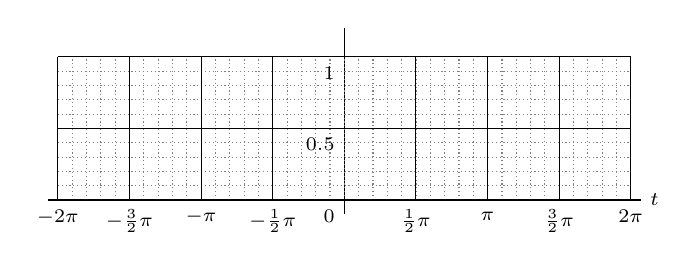
\begin{tikzpicture}[xscale=0.579, yscale=1.818]
	\def\piv{3.1416}
	\coordinate (o) at (0,0);
	\draw (o) ++(-6.5,0) -- ++(13, 0) node [anchor=west] {\scriptsize $t$};
	\draw (o) ++(0,-0.1) -- ++(0, 1.3);% node [anchor=south] {\scriptsize $x(t)$};	
	
	\foreach \y in {0, 0.1, ..., 1}
	{
		\draw[thin, gray, densely dotted] (-2*\piv, \y) -- ++(4*\piv, 0);
	}	

	\foreach \x in {- 6.2832, -5.9690, ...,  6.2832}
	{
		\draw[thin, gray, densely dotted]  (\x, 0) -- ++(0,1);
	}		
	
	
	\foreach \x/\v in {-2*\piv/-2, -1.5*\piv/-\frac{3}{2}, -1*\piv/-, -0.5*pi/{-\frac{1}{2}},  0.5*\piv/\frac{1}{2}, 1*\piv/, 1.5*\piv/\frac{3}{2}, 2*\piv/2}
	{
		\draw (\x, 0) -- ++(0,1);
		\node at (\x, 0) [anchor=north, minimum height=0.4cm] {\scriptsize $ \v\pi$};
	}
	\foreach \y in {0, 0.5, 1}
	{
		\draw (-2*\piv, \y) -- ++(4*\piv, 0);
		\node  at (0, \y) [anchor=north east] {\scriptsize $ \y $};
	}

\end{tikzpicture}  & 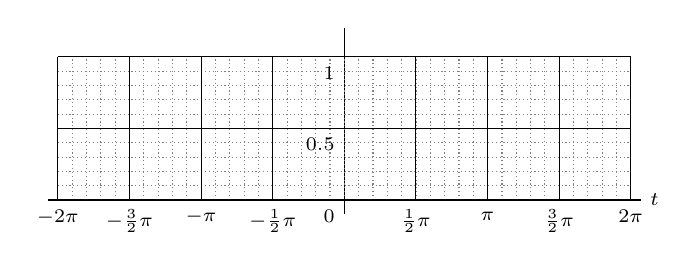
\begin{tikzpicture}[xscale=0.579, yscale=1.818]
	\def\piv{3.1416}
	\coordinate (o) at (0,0);
	\draw (o) ++(-6.5,0) -- ++(13, 0) node [anchor=west] {\scriptsize $t$};
	\draw (o) ++(0,-0.1) -- ++(0, 1.3);% node [anchor=south] {\scriptsize $x(t)$};	
	
	\foreach \y in {0, 0.1, ..., 1}
	{
		\draw[thin, gray, densely dotted] (-2*\piv, \y) -- ++(4*\piv, 0);
	}	

	\foreach \x in {- 6.2832, -5.9690, ...,  6.2832}
	{
		\draw[thin, gray, densely dotted]  (\x, 0) -- ++(0,1);
	}		
	
	
	\foreach \x/\v in {-2*\piv/-2, -1.5*\piv/-\frac{3}{2}, -1*\piv/-, -0.5*pi/{-\frac{1}{2}},  0.5*\piv/\frac{1}{2}, 1*\piv/, 1.5*\piv/\frac{3}{2}, 2*\piv/2}
	{
		\draw (\x, 0) -- ++(0,1);
		\node at (\x, 0) [anchor=north, minimum height=0.4cm] {\scriptsize $ \v\pi$};
	}
	\foreach \y in {0, 0.5, 1}
	{
		\draw (-2*\piv, \y) -- ++(4*\piv, 0);
		\node  at (0, \y) [anchor=north east] {\scriptsize $ \y $};
	}

\end{tikzpicture}  \\
    \end{tabular}



   %\tikz \draw (0,0) rectangle (6in, 1.5in);





\item Plot the real part of
    $
        x(t) = Ce^{at}
    $
    where
    $
        C = |C|e^{j\theta}
    $
    and
    $
        a = r + j\omega_0
    $.
    \mks{2}

  \noindent  \begin{tabular}{cc}
        $|C| = 0.15$, $\theta = 0$, $\omega_0 = 2\:\mathrm{rad/s}$, $r = 0.3$  & $|C| = 0.15$, $\theta = 0$, $\omega_0 = 2\:\mathrm{rad/s}$, $r = -0.3$\\
        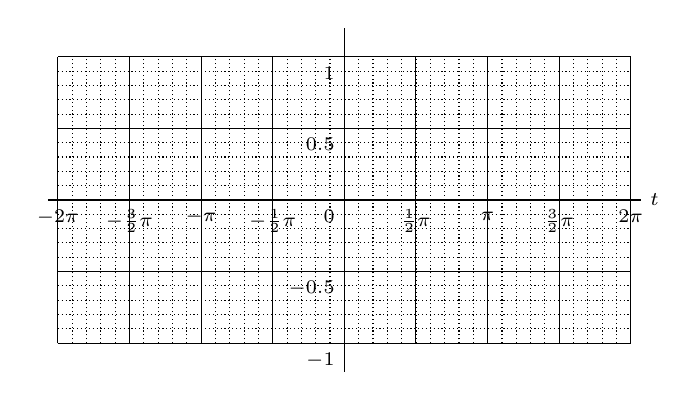
\begin{tikzpicture}[xscale=0.579, yscale=1.818]
	\def\piv{3.1416}
	\coordinate (o) at (0,0);
	\draw (o) ++(-6.5,0) -- ++(13, 0) node [anchor=west] {\scriptsize $t$};
	\draw (o) ++(0,-1.2) -- ++(0, 2.4);% node [anchor=south] {\scriptsize $x(t)$};	
	
	\foreach \y in {-1, -0.9, ..., 1}
	{
		\draw[thin, densely dotted] (-2*\piv, \y) -- ++(4*\piv, 0);
	}	

	\foreach \x in {- 6.2832, -5.9690, ...,  6.2832}
	{
		\draw[thin, densely dotted]  (\x, -1) -- ++(0,2);
	}		
	
	
	\foreach \x/\v in {-2*\piv/-2, -1.5*\piv/-\frac{3}{2}, -1*\piv/-, -0.5*pi/{-\frac{1}{2}},  0.5*\piv/\frac{1}{2}, 1*\piv/, 1.5*\piv/\frac{3}{2}, 2*\piv/2}
	{
		\draw (\x, -1) -- ++(0,2);
		\node at (\x, 0) [anchor=north, minimum height=0.4cm] {\scriptsize $ \v\pi$};
	}
	\foreach \y in {-1, -0.5, 0, 0.5, 1}
	{
		\draw (-2*\piv, \y) -- ++(4*\piv, 0);
		\node  at (0, \y) [anchor=north east] {\scriptsize $ \y $};
	}

\end{tikzpicture}  & 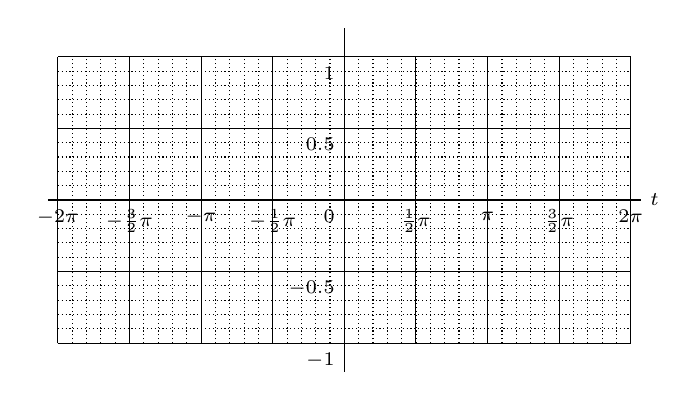
\begin{tikzpicture}[xscale=0.579, yscale=1.818]
	\def\piv{3.1416}
	\coordinate (o) at (0,0);
	\draw (o) ++(-6.5,0) -- ++(13, 0) node [anchor=west] {\scriptsize $t$};
	\draw (o) ++(0,-1.2) -- ++(0, 2.4);% node [anchor=south] {\scriptsize $x(t)$};	
	
	\foreach \y in {-1, -0.9, ..., 1}
	{
		\draw[thin, densely dotted] (-2*\piv, \y) -- ++(4*\piv, 0);
	}	

	\foreach \x in {- 6.2832, -5.9690, ...,  6.2832}
	{
		\draw[thin, densely dotted]  (\x, -1) -- ++(0,2);
	}		
	
	
	\foreach \x/\v in {-2*\piv/-2, -1.5*\piv/-\frac{3}{2}, -1*\piv/-, -0.5*pi/{-\frac{1}{2}},  0.5*\piv/\frac{1}{2}, 1*\piv/, 1.5*\piv/\frac{3}{2}, 2*\piv/2}
	{
		\draw (\x, -1) -- ++(0,2);
		\node at (\x, 0) [anchor=north, minimum height=0.4cm] {\scriptsize $ \v\pi$};
	}
	\foreach \y in {-1, -0.5, 0, 0.5, 1}
	{
		\draw (-2*\piv, \y) -- ++(4*\piv, 0);
		\node  at (0, \y) [anchor=north east] {\scriptsize $ \y $};
	}

\end{tikzpicture}  \\
    \end{tabular}


\item Plot the real part of
    $
        x[n] = C\alpha^n
    $
    where
    $
        C = |C|e^{j\theta}
    $
    and
    $
        \alpha = |\alpha|e^{j\omega_0}
    $.
    \mks{3}

  \noindent  \begin{tabular}{cc}
        $|C| = 0.15$, $\alpha = 0.9$, $\omega_0 = 2\pi/16$, $\theta = 0$  & $|C| = 0.15$, $\alpha = 1.9$, $\omega_0 = 2\pi/16$, $\theta = 0$  \\
        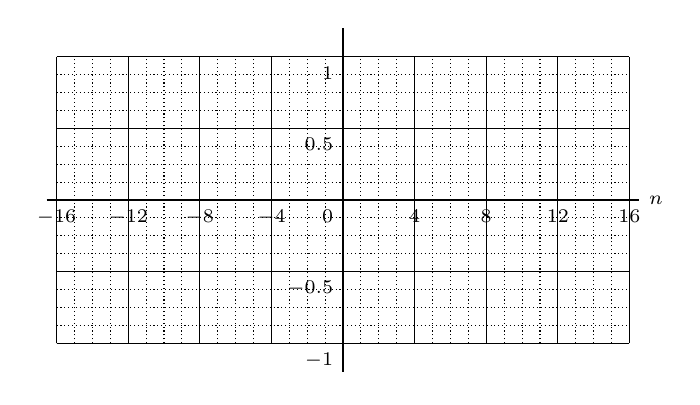
\begin{tikzpicture}[xscale=0.579, yscale=1.818]
	\def\piv{3.1416}
	\coordinate (o) at (0,0);
	\draw (o) ++(-6.5,0) -- ++(13, 0) node [anchor=west] {\scriptsize $n$};
	\draw (o) ++(0,-1.2) -- ++(0, 2.4);% node [anchor=south] {\scriptsize $x[n]$};	
	
	\foreach \y in {-1, -0.875, ..., 1}
	{
		\draw[thin, densely dotted] (-2*\piv, \y) -- ++(4*\piv, 0);
	}	

	\foreach \x in {- 6.2832, -5.8905, ...,  6.2832}
	{
		\draw[thin, densely dotted]  (\x, -1) -- ++(0,2);
	}		
	
	
	\foreach \x/\v in {-2*\piv/-16, -1.5*\piv/-12, -1*\piv/-8, -0.5*pi/-4,  0.5*\piv/4, 1*\piv/8, 1.5*\piv/12, 2*\piv/16}
	{
		\draw (\x, -1) -- ++(0,2);
		\node at (\x, 0) [anchor=north, minimum height=0.4cm] {\scriptsize $ \v$};
	}
	\foreach \y in {-1, -0.5, 0, 0.5, 1}
	{
		\draw (-2*\piv, \y) -- ++(4*\piv, 0);
		\node  at (0, \y) [anchor=north east] {\scriptsize $ \y $};
	}

\end{tikzpicture}  & 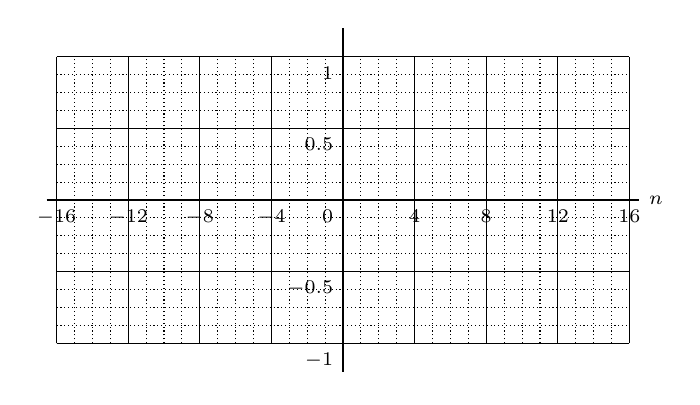
\begin{tikzpicture}[xscale=0.579, yscale=1.818]
	\def\piv{3.1416}
	\coordinate (o) at (0,0);
	\draw (o) ++(-6.5,0) -- ++(13, 0) node [anchor=west] {\scriptsize $n$};
	\draw (o) ++(0,-1.2) -- ++(0, 2.4);% node [anchor=south] {\scriptsize $x[n]$};	
	
	\foreach \y in {-1, -0.875, ..., 1}
	{
		\draw[thin, densely dotted] (-2*\piv, \y) -- ++(4*\piv, 0);
	}	

	\foreach \x in {- 6.2832, -5.8905, ...,  6.2832}
	{
		\draw[thin, densely dotted]  (\x, -1) -- ++(0,2);
	}		
	
	
	\foreach \x/\v in {-2*\piv/-16, -1.5*\piv/-12, -1*\piv/-8, -0.5*pi/-4,  0.5*\piv/4, 1*\piv/8, 1.5*\piv/12, 2*\piv/16}
	{
		\draw (\x, -1) -- ++(0,2);
		\node at (\x, 0) [anchor=north, minimum height=0.4cm] {\scriptsize $ \v$};
	}
	\foreach \y in {-1, -0.5, 0, 0.5, 1}
	{
		\draw (-2*\piv, \y) -- ++(4*\piv, 0);
		\node  at (0, \y) [anchor=north east] {\scriptsize $ \y $};
	}

\end{tikzpicture}  \\
    \end{tabular}






   %\tikz \draw (0,0) rectangle (6in, 1.5in);

\end{enumerate}





\end{document} 